\documentclass[12pt]{article}
\usepackage[margin=1in]{geometry}
\usepackage{amsmath,amssymb,amsthm}
\usepackage{graphicx}
\usepackage{hyperref}
\usepackage{xcolor}
\newlength\tindent
\setlength{\parindent}{0pt}
\setlength{\tindent}{\parindent}
\renewcommand{\indent}{\hspace*{\tindent}}


\usepackage{subcaption}

\title{Phase 03}
\author{Tamzeed Elahi}
\date{\today}



\begin{document}
\maketitle

Most recent version of this document can be found \href{https://github.com/tamzeed-toha/Nonlinear_and_Data_Driven_Estimation/blob/main/write_ups/phase_02.pdf}{\textcolor{blue}{here}}. 

Code for this project can be found \href{https://github.com/tamzeed-toha/Nonlinear_and_Data_Driven_Estimation/blob/main/project/phase_02.ipynb}{\textcolor{blue}{here}}.

\section*{Project Description}
The problem I am interested for the class project is a system identification problem for a 2D quadrotor system. In the context of this course, the observability of this system will be evaluated; especially for estimating the input matrix which is unknown. 
\begin{align*}
    \dot{x} &= Ax + Bu + w \\
    y &= Cx + v
\end{align*} 
Here, the B matrix is unknown. \\\\
Ultimately, we would be able to estimate the B matrix using the observability matrix and consider the feasibility of a quadrotor system with additional controls (sliding/tilting) like \cite{Nemati2014}. 

\section*{Abstract}



\section*{Introduction}



\section*{Analytical model of quadrotor system}
\begin{figure}[h!]
    \begin{subfigure}[t]{0.5\textwidth}
        \centering
        \includegraphics[width=5cm]{figures/model_diagram.png}
        \caption{Quadrotor system \cite{model_diagram}}
        \label{fig:01}
    \end{subfigure}
    \hfill
    \begin{subfigure}[t]{0.5\textwidth}
        \centering
        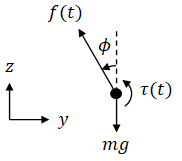
\includegraphics[width=5cm]{figures/free_body_diagram.png}
        \caption{Free body diagram \cite{model_diagram}}
        \label{fig:02}
    \end{subfigure}
\end{figure}
% \includegraphics[width=5cm]{model_diagram.png}

The state space model of a quadrotor system can be found in various literature\cite{K2019}\cite{Schreier2012}. For the class project, I will be using a simplified 2D model (only the y and z coordinates). The dynamic equation of the system can be estimated using Newton's second law of motion.
\begin{align*}
    \ddot{y} &= -\frac{1}{m}u_1(t) \sin{\phi} \\
    \ddot{z} &= -g + \frac{1}{m}u_1(t) \cos{\phi} \\ 
    \ddot{\phi} &= \frac{1}{I_{xx}}u_2(t) \\
\end{align*}
I assumed only two inputs (force and torque) are present in the system. Their relation with the states are nonlinear though it can be linearized with $\phi \approx 0$. It would be more interesting if the inputs are not forces and torques but rotor speeds. \\\\
States are: $x = [\dot{\theta}, \theta, \dot{x}, x, \dot{z}, z]^T$ \\
For now the output matrix-$C$ is considered to be an identity matrix. So, the system assumed to have a GPS and IMU sensors for full state estimation.

inputs are:
\begin{align*}
    u_1(t) &= F \\
    u_2(t) &= \tau
\end{align*}
matrices in continuous form:
\begin{align*}
    A &= \begin{bmatrix}
        0 & 1 & 0 & 0 & 0 & 0 \\
        0 & 0 & 0 & 0 & 0 & 0 \\
        0 & 0 & 0 & 1 & 0 & 0 \\
        0 & 0 & 0 & 0 & 0 & 0 \\
        0 & 0 & 0 & 0 & 0 & 1 \\
        0 & 0 & 0 & 0 & 0 & 0
    \end{bmatrix} \\
    B &= \begin{bmatrix}
        0 & 0 \\
        0 & \frac{1}{I_{xx}} \\
        0 & 0 \\
        - \frac{1}{m} \sin{\theta} & 0 \\
        0 & 0 \\
        \frac{1}{m} \cos{\theta} & 0 \\
    \end{bmatrix} \\
\end{align*}

\section*{Organized dynamic equations:}

States:
\begin{align*}
    \vec{x} &= \begin{bmatrix}
        \colorbox{yellow}{$\dot{\theta}$} \\
        \colorbox{yellow}{$\theta$} \\
        \colorbox{yellow}{$\dot{x}$} \\
        \colorbox{yellow}{$x$} \\
        \colorbox{yellow}{$\dot{z}$} \\
        \colorbox{yellow}{$z$} \\
        \hline
        \colorbox{pink}{$\beta_1$} \\
        \colorbox{pink}{$\beta_2$} \\
        \colorbox{pink}{$\beta_3$} \\
    \end{bmatrix}
\end{align*}

Dynamic equations:
\begin{align*}
    \dot{\vec{x}} &= \begin{bmatrix}
        \colorbox{pink}{$\beta_1$} \colorbox{lime}{$u_2$} \\
        \colorbox{yellow}{$\dot{\theta}$} \\
        \colorbox{pink}{$\beta_2$} \colorbox{lime}{$u_1$} \sin{\colorbox{yellow}{$\theta$}} \\ 
        \colorbox{yellow}{$\dot{x}$} \\
        -\colorbox{cyan}{g}+\colorbox{pink}{$\beta_3$} \colorbox{lime}{$u_1$} \cos{\colorbox{yellow}{$\theta$}} \\
        \colorbox{yellow}{$\dot{z}$} \\
        \hline
        0 \\
        0 \\
        0 \\
    \end{bmatrix} \\
    &= \begin{bmatrix}
            0 \\
            \colorbox{yellow}{$\dot{\theta}$} \\
            0 \\
            \colorbox{yellow}{$\dot{x}$} \\
            -\colorbox{cyan}{g} \\
            \colorbox{yellow}{$\dot{z}$} \\
            \hline
            0 \\
            0 \\
            0 \\
        \end{bmatrix} +  \begin{bmatrix}
            0 \\
            0 \\
            \colorbox{pink}{$\beta_2$} \sin{\colorbox{yellow}{$\theta$}} \\
            0 \\
            \colorbox{pink}{$\beta_3$} \cos{\colorbox{yellow}{$\theta$}} \\
            0 \\
            \hline
            0 \\
            0 \\
            0 \\
        \end{bmatrix} \colorbox{lime}{$u_1$} +  \begin{bmatrix}
            \colorbox{pink}{$\beta_1$} \\
            0 \\
            0 \\
            0 \\
            0 \\
            0 \\    
            \hline        
            0 \\
            0 \\
            0 \\
        \end{bmatrix} \colorbox{lime}{$u_2$} \\
    &= \begin{bmatrix}
        0 \\
        \colorbox{yellow}{$\dot{\theta}$} \\
        0 \\
        \colorbox{yellow}{$\dot{x}$} \\
        -\colorbox{cyan}{g} \\
        \colorbox{yellow}{$\dot{z}$} \\
        \hline
        0 \\
        0 \\
        0 \\
    \end{bmatrix} +  \begin{bmatrix}
        0 \\
        0 \\
        \colorbox{pink}{$\beta_2$} \\
        0 \\
        \colorbox{pink}{$\beta_3$} \\
        0 \\
        \hline
        0 \\
        0 \\
        0 \\
    \end{bmatrix} \colorbox{lime}{$\tilde{u}_1$} + \begin{bmatrix}
        \colorbox{pink}{$\beta_1$} \\
        0 \\
        0 \\
        0 \\
        0 \\
        0 \\ 
        \hline
        0 \\
        0 \\
        0 \\
    \end{bmatrix} \colorbox{lime}{$u_2$} 
\end{align*}

where, 
\begin{align*}
    \tilde{u}_1 &= \begin{bmatrix}
        0 \\
        0 \\
        \sin{\colorbox{yellow}{$\theta$}} \\
        0 \\
        \cos{\colorbox{yellow}{$\theta$}} \\
        0 \\
        \hline
        0 \\
        0 \\
        0 \\
    \end{bmatrix} u_1
\end{align*}

known constants: \colorbox{cyan}{$g$} = 9.81 $m/s^2$ \\

Measurement matrix: I do not have any non-linearity in the measurement matrix. It is currently assumed to be an identity matrix. I can certainly get by with fewer sensors but the beta values need direct measurement as of now.

\pagebreak
\section*{Results:}

\subsection*{Linear case:}
The nonlinearity of this system is due to the input matrix. The input matrix is a function of the states. So, the system is nonlinear. If we consider the unknown parameters of input matrix as a part of the state, then our new A matrix would be:

\begin{align*}
    \dot{x} &= \begin{bmatrix}
        0 & 1 & 0 & 0 & 0 & 0 & 0 & 0 & 0 \\
        0 & 0 & 0 & 0 & 0 & 0 & 0 & 0 & 0 \\
        0 & 0 & 0 & 1 & 0 & 0 & 0 & 0 & 0 \\
        0 & 0 & 0 & 0 & 0 & 0 & 0 & 0 & 0 \\
        0 & 0 & 0 & 0 & 0 & 1 & 0 & 0 & 0 \\
        0 & 0 & 0 & 0 & 0 & 0 & 0 & 0 & 0 \\
        0 & 0 & 0 & 0 & 0 & 0 & 0 & 0 & 0 \\
        0 & 0 & 0 & 0 & 0 & 0 & 0 & 0 & 0 \\
        0 & 0 & 0 & 0 & 0 & 0 & 0 & 0 & 0 \\
    \end{bmatrix} \begin{bmatrix}
        \dot{\theta} \\
        \theta \\
        \dot{x} \\
        x \\
        \dot{z} \\
        z \\
        \beta_1 \\
        \beta_2 \\
        \beta_3 \\
    \end{bmatrix} + \begin{bmatrix}
        0 & 0 \\
        0 & \frac{1}{I_{xx}} \\
        0 & 0 \\
        - \frac{1}{m} \sin{\theta} & 0 \\
        0 & 0 \\
        \frac{1}{m} \cos{\theta} & 0 \\
        0 & 0 \\
        0 & 0 \\
        0 & 0 \\
    \end{bmatrix} \begin{bmatrix}
        F \\
        \tau \\
    \end{bmatrix} 
\end{align*}

Our first task would be to estimate the unknown parameters of the input matrix knowing input matrix using an estimator (Kalman filter). As the A matrix is already linear, we have to discretize it first and then apply the Kalman filter. For our problem, lets break down the input matrix into two parts. One part is known and the other part is unknown.


\begin{align*}
    B_{n \times m} &= B^{0}_{n \times k} B^{1}_{k \times m} \\ 
    \text{so,}  \\
    \dot{x} &= Ax + B^{0} B^{1} u \\
    &= Ax + B^{0} u_{B} \\
    y &= Cx 
\end{align*}
where $B^{0}$ is unknown and $B^{1}$ is known. Here, $B^{0}$ is a row vector but it can be a matrix if the inputs are not linearly independent.

Contiuous form of the system:
\begin{align*}
    \dot{x} &= Ax + B^{0} u_{B} \\
    &= \begin{bmatrix}
        0 & 1 & 0 & 0 & 0 & 0 & 0 & 0 & 0 \\
        0 & 0 & 0 & 0 & 0 & 0 & 0 & 0 & 0 \\
        0 & 0 & 0 & 1 & 0 & 0 & 0 & 0 & 0 \\
        0 & 0 & 0 & 0 & 0 & 0 & 0 & 0 & 0 \\
        0 & 0 & 0 & 0 & 0 & 1 & 0 & 0 & 0 \\
        0 & 0 & 0 & 0 & 0 & 0 & 0 & 0 & 0 \\
        0 & 0 & 0 & 0 & 0 & 0 & 0 & 0 & 0 \\
        0 & 0 & 0 & 0 & 0 & 0 & 0 & 0 & 0 \\
        0 & 0 & 0 & 0 & 0 & 0 & 0 & 0 & 0 \\
    \end{bmatrix} \begin{bmatrix}
        \dot{\theta} \\
        \theta \\
        \dot{x} \\
        x \\
        \dot{z} \\
        z \\
        \beta_1 \\
        \beta_2 \\
        \beta_3 \\
    \end{bmatrix} + \begin{bmatrix}
        0 \\ \frac{1}{I_{xx}} \\ 0 \\ -\frac{1}{m} \\ 0 \\ \frac{1}{m} \\  0 \\ 0 \\ 0
        \end{bmatrix}^{T} \begin{bmatrix}
            0 & 0 \\
            0 & 1 \\
            0 & 0 \\
            \sin{\theta} & 0 \\
            0 & 0 \\
            \cos{\theta} & 0 \\
            0 & 0 \\
            0 & 0 \\
            0 & 0 \\
        \end{bmatrix} \begin{bmatrix}
            F \\
            \tau \\
        \end{bmatrix}
\end{align*}
We know, the continuous form of the system can be discretized using the following equation:
\begin{align*}
    A_d &= e^{A \Delta t}  = \phi(\Delta t) \\
    B_d &= (A_d - I) A^{-1} B \\
    C_d &= C
\end{align*}
In this case, A matrix is singular so we can't use the above equation. We can use the following equation to discretize the system:
\begin{align*}
    A_d &= I + A \Delta t + \frac{A^2 \Delta t^2}{2} + \frac{A^3 \Delta t^3}{6} + \ldots \\
    B_d &= \int_{0}^{\Delta t} e^{A \tau} d\tau B \\
    C_d &= C
\end{align*}
The discretized form of the system is:
\begin{align*}
    A_d &= \begin{bmatrix}
        1 & \Delta t & 0 & 0 & 0 & 0 & 0 & 0 & 0 \\
        0 & 1 & 0 & 0 & 0 & 0 & 0 & 0 & 0 \\
        0 & 0 & 1 & \Delta t & 0 & 0 & 0 & 0 & 0 \\
        0 & 0 & 0 & 1 & 0 & 0 & 0 & 0 & 0 \\
        0 & 0 & 0 & 0 & 1 & \Delta t & 0 & 0 & 0 \\
        0 & 0 & 0 & 0 & 0 & 1 & 0 & 0 & 0 \\
        0 & 0 & 0 & 0 & 0 & 0 & 1 & 0 & 0 \\
        0 & 0 & 0 & 0 & 0 & 0 & 0 & 1 & 0 \\
        0 & 0 & 0 & 0 & 0 & 0 & 0 & 0 & 1 \\
    \end{bmatrix} \\
\end{align*}


\color{red}
Estimation of $B_d$ matrix is a bit tricky because of the singularity of the A matrix. I have estimated the B matrix in two methods:
\begin{enumerate}
    \item Using pseudo-inverse (Moore-Penrose inverse) I got a zero matrix.
    \item Using the integral equation, I got a non-zero matrix. For $\Delta t = 0.1$, the B matrix is: $B_d = \begin{bmatrix}   6.25e-01 \\  1.25e+01 \\ -1.00e-02 \\ -2.00e-01 \\ 1.00e-02 \\ 2.00e-01 \\
        0.00e+00 \\  0.00e+00 \\  0.00e+00 \end{bmatrix}$
\end{enumerate}

\color{black}



Now, we divert our attention to the measurement matrix of the system. The observability of the system is dependent on the measurement matrix. We have to design the measurement matrix in such a way that the system is observable. 

\subsubsection*{Observability}
The observability of the system can be evaluated using the observability matrix. The system is observable if the rank of the observability matrix is equal to the number of states. The observability matrix is given by:
\begin{align*}
    O = \begin{bmatrix}
        C \\
        CA \\
        CA^2 \\
        \vdots \\
        CA^{n-1}
    \end{bmatrix}
\end{align*}

\subsection*{Designing a measurement matrix}
Let's consider the measurement matrix as an identity matrix. 
\begin{align*}
    C &= I
\end{align*}
This makes the system observable (rank = 9). We can get by with lower number of sensors. But, as the beta values don't really have a dynamics, they need direct measurement for estimation. At least for the linear case.

The measurement plot is given below:
\begin{figure}[h!]
    \centering
    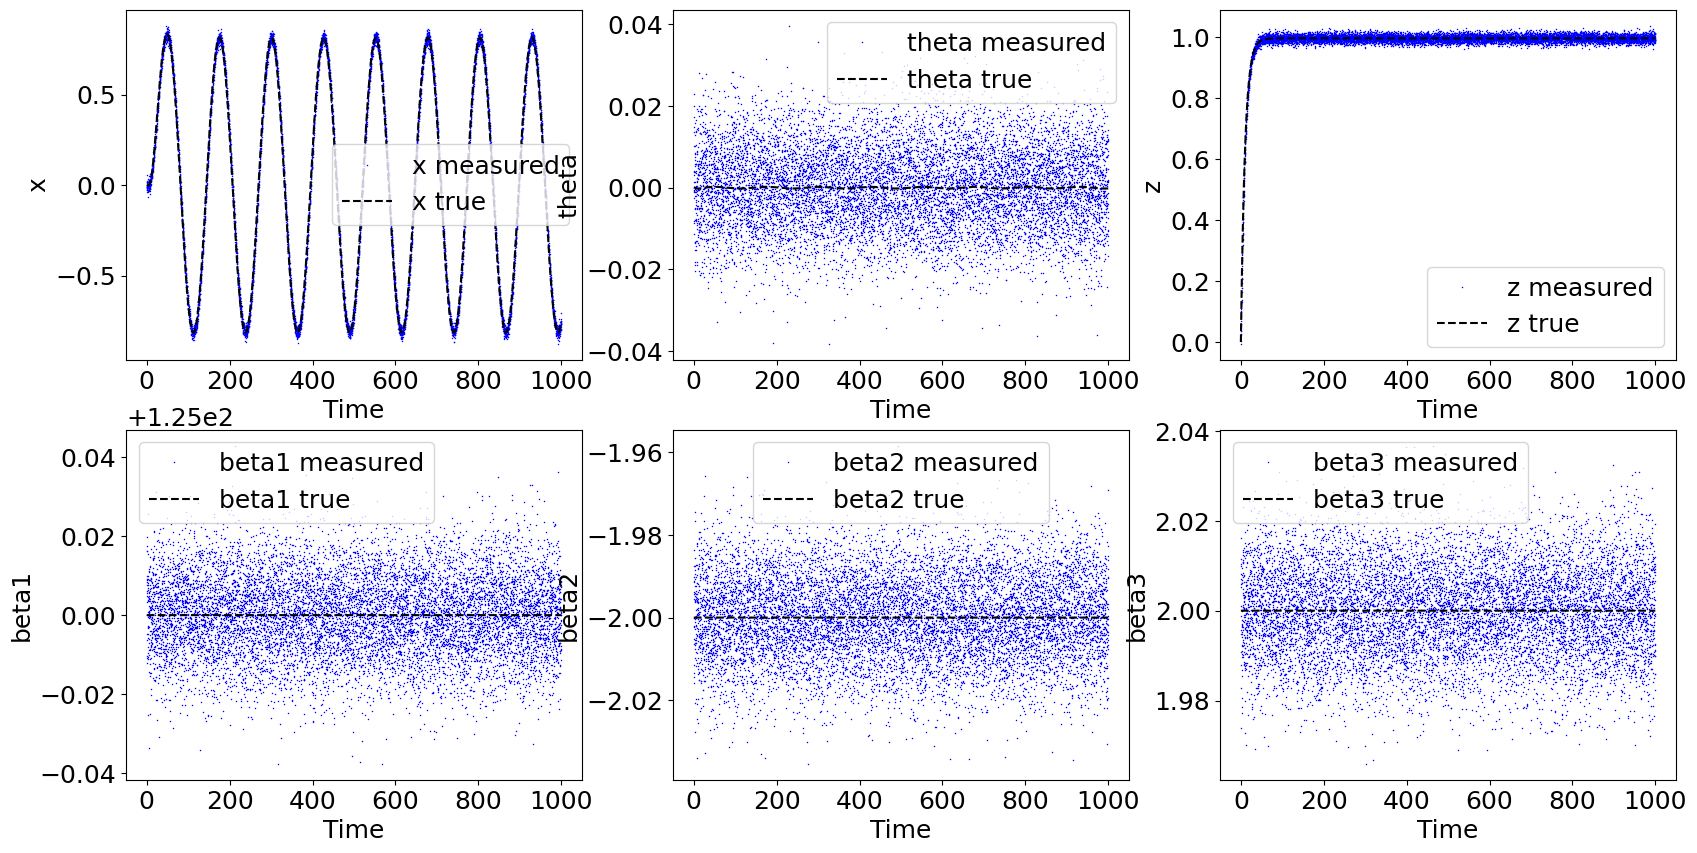
\includegraphics[width=10cm]{figures/phase_02_measurement1.png}
    \caption{Measurement plot}
    \label{fig:03}
\end{figure}
The estimator was able to estimate the states and the unknown parameters of the input matrix. The plot of the estimated states and the true states are given below:
\begin{figure}[h!]
    \centering
    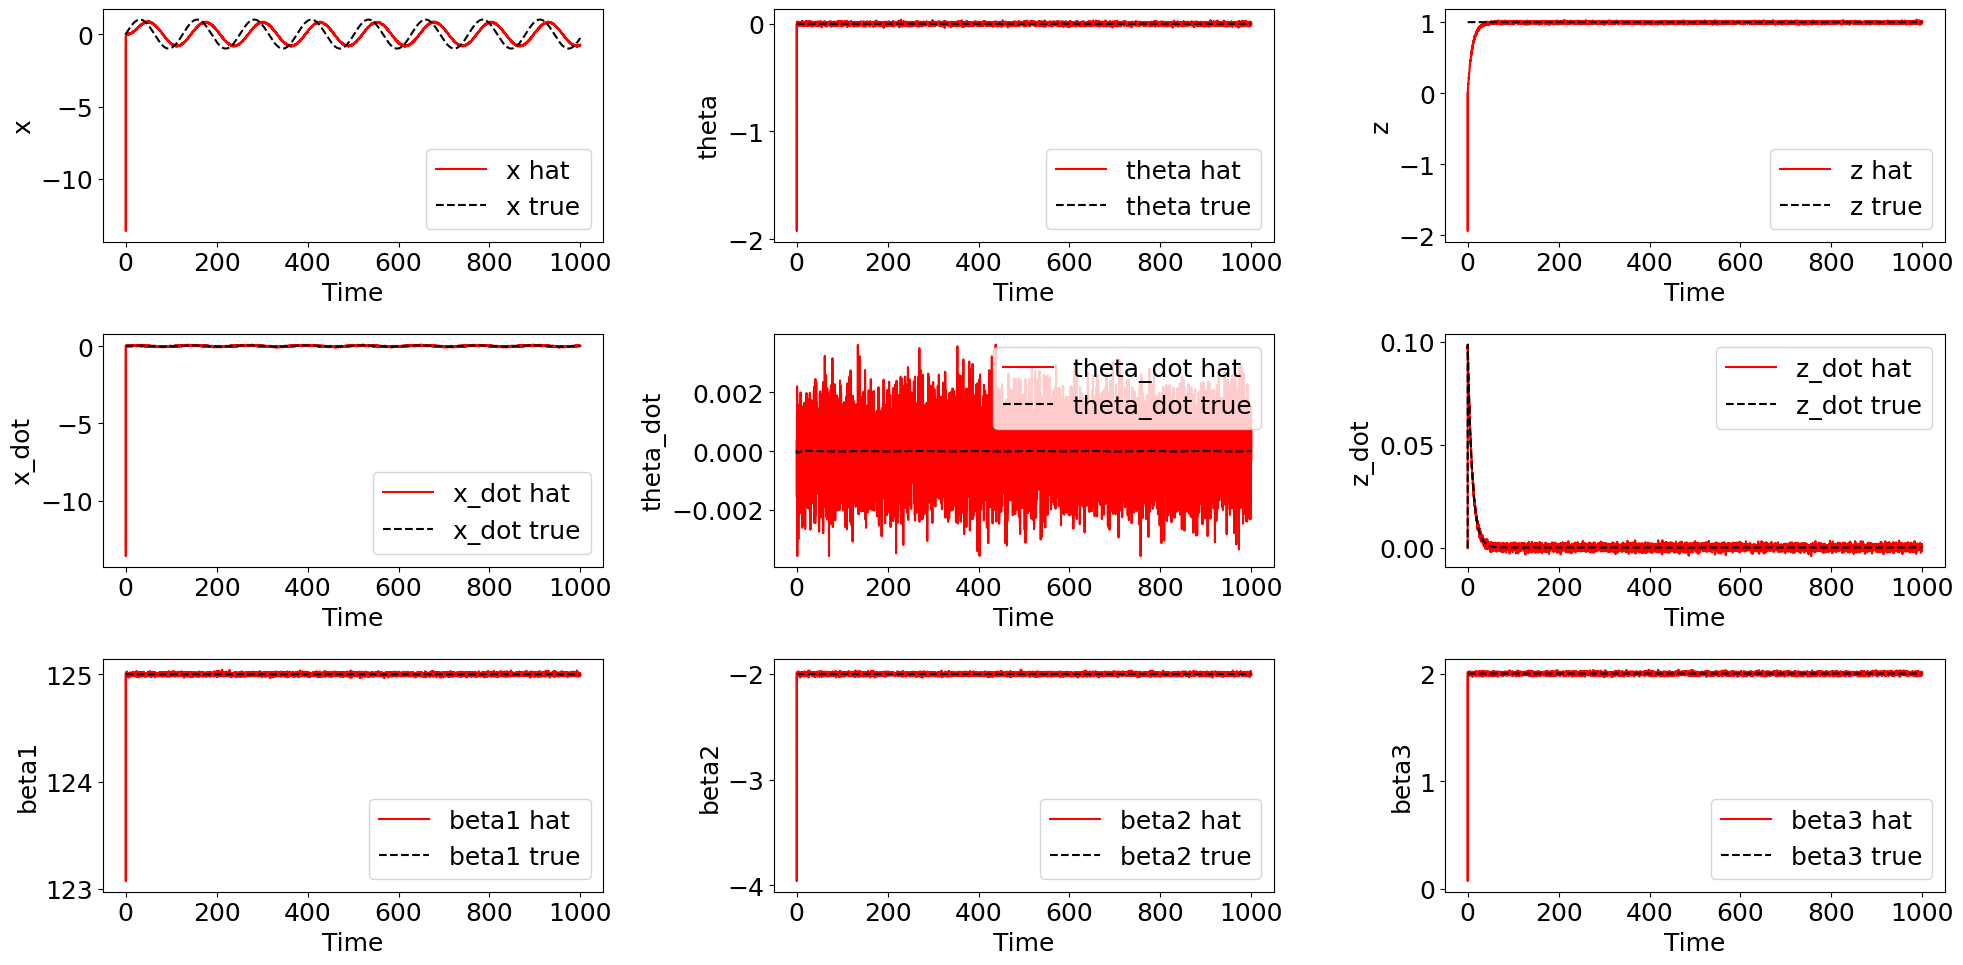
\includegraphics[width=10cm]{figures/phase_02_states1.png}
    \caption{State estimation}
    \label{fig:04}
\end{figure}

\section*{Conclusion}

\pagebreak
\bibliographystyle{plain}
\bibliography{phase0}









\end{document}